\section{Bối cảnh bài toán}

Minesweeper là một trò chơi giải đố, diễn ra trên một bảng ô vuông kích thước R×C. Một số ô chứa mìn được đặt ẩn bên dưới, và người chơi sẽ mở từng ô để tìm vùng an toàn, dựa vào các con số cho biết có bao nhiêu mìn nằm xung quanh.

Nếu nhìn dưới góc độ cấu trúc dữ liệu, bàn chơi thực chất là một lưới 2D, nơi mỗi ô có thể xem như một “điểm” kết nối với tối đa 8 ô xung quanh nó. Khi vận hành trò chơi, hệ thống phải xử lý các thao tác mở ô, kiểm tra mìn và đặc biệt là cơ chế mở lan những vùng trống. Vì vậy, phía sau một trò chơi tưởng chừng đơn giản là cả một bài toán về duyệt đồ thị và quản lý trạng thái.

\begin{center}
\begin{figure}[H]
    \centering
    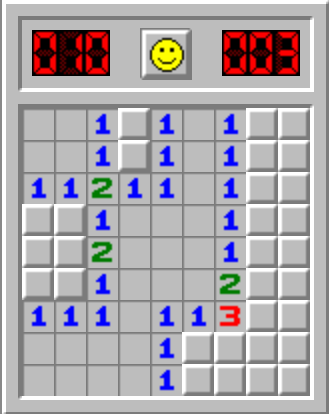
\includegraphics[width=0.25\linewidth]{../../images/ai/ms.png}
    \vspace{0.5cm}
    \caption{Hình ảnh của game Minesweeper}
\end{figure}
\end{center}